\chapter{Experimentación}

% ------------------------------------------------------------------------------------------------------------

\section{Protocolo de validación experimental}

Como se ha comentado anteriormente, se han proporcionado los datos ya dividos en conjunto de entrenamiento
(\textit{train}) y de test, para evitar problemas asociados al \textit{data snooping}. El 
\textbf{\textit{data snooping}} ocurre cuando información del conjunto de test se filtra, directa o 
indirectamente, en el proceso de entrenamiento del modelo, lo que puede llevar a una sobreestimación del 
rendimiento y a modelos que generalizan pobremente en datos nuevos.




Debemos ser cuidadosos a la hora de tratar los datos en test, no debemos ... la variable de edad de los 
individuos, ya que es el target en nuestro problema de regresión, y cualquier ... puede ... Esto se conoce
como data snooping





Para valorar los resultados obtenidos en los experimentos realizados se han divido los datos de 
entrenamiento en \textit{train} y \textit{validation}. 

Se consideró la validación cruzada (\textit{cross-validation}), pero 
\textit{data split}


\begin{figure}[h]
    \centering
    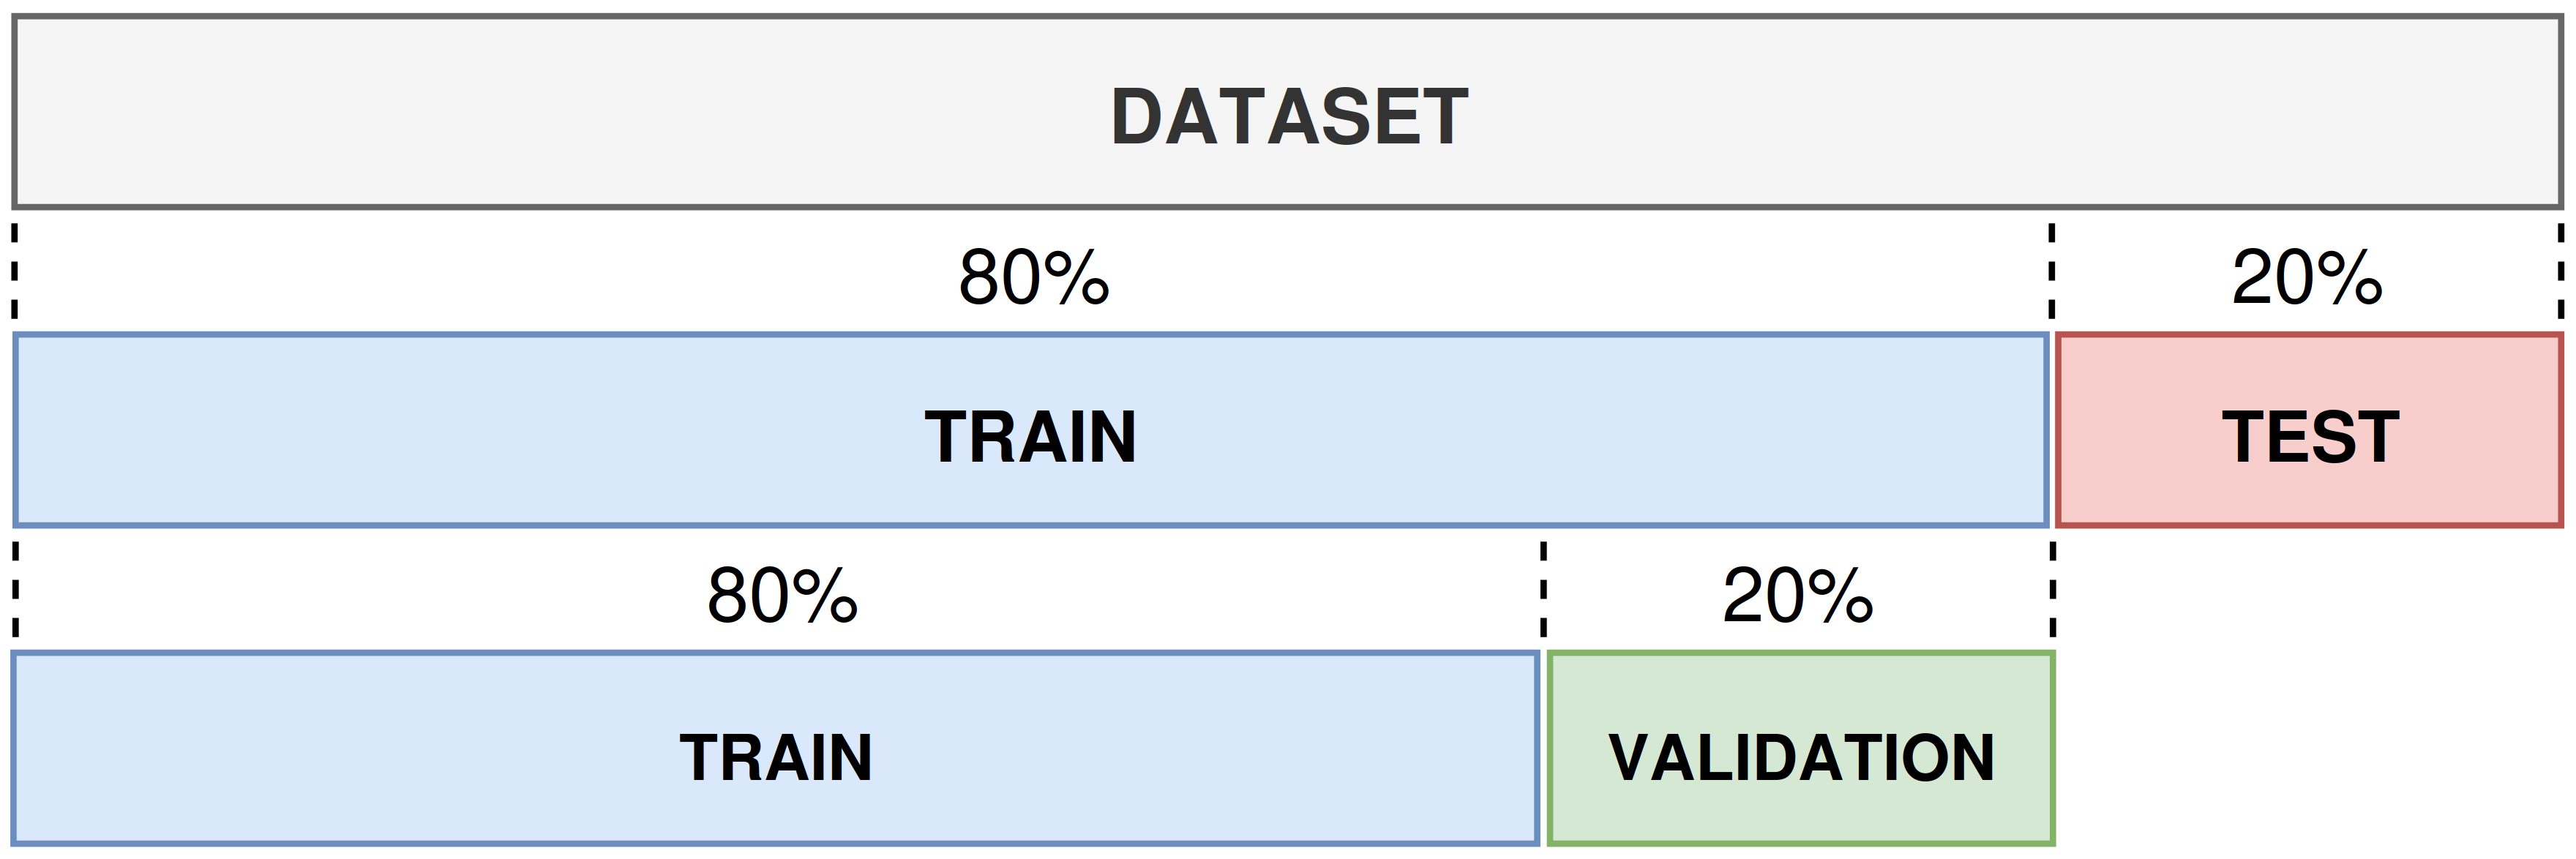
\includegraphics[width=\textwidth]{capitulos/cap_04/imagenes/data_split_base.png}
    \caption[
        Diagrama de división del \textit{dataset} en \textit{train}, \textit{validation} y \textit{test}.
    ]{
        Diagrama de división del \textit{dataset} en \textit{train}, \textit{validation} y \textit{test}. 
        Elaboración propia.
    } 
    \label{fig:data_split_base}
\end{figure}

Sin embargo, aquellos métodos de predicción conformal requieren de una fracción 

\begin{figure}[h]
    \centering
    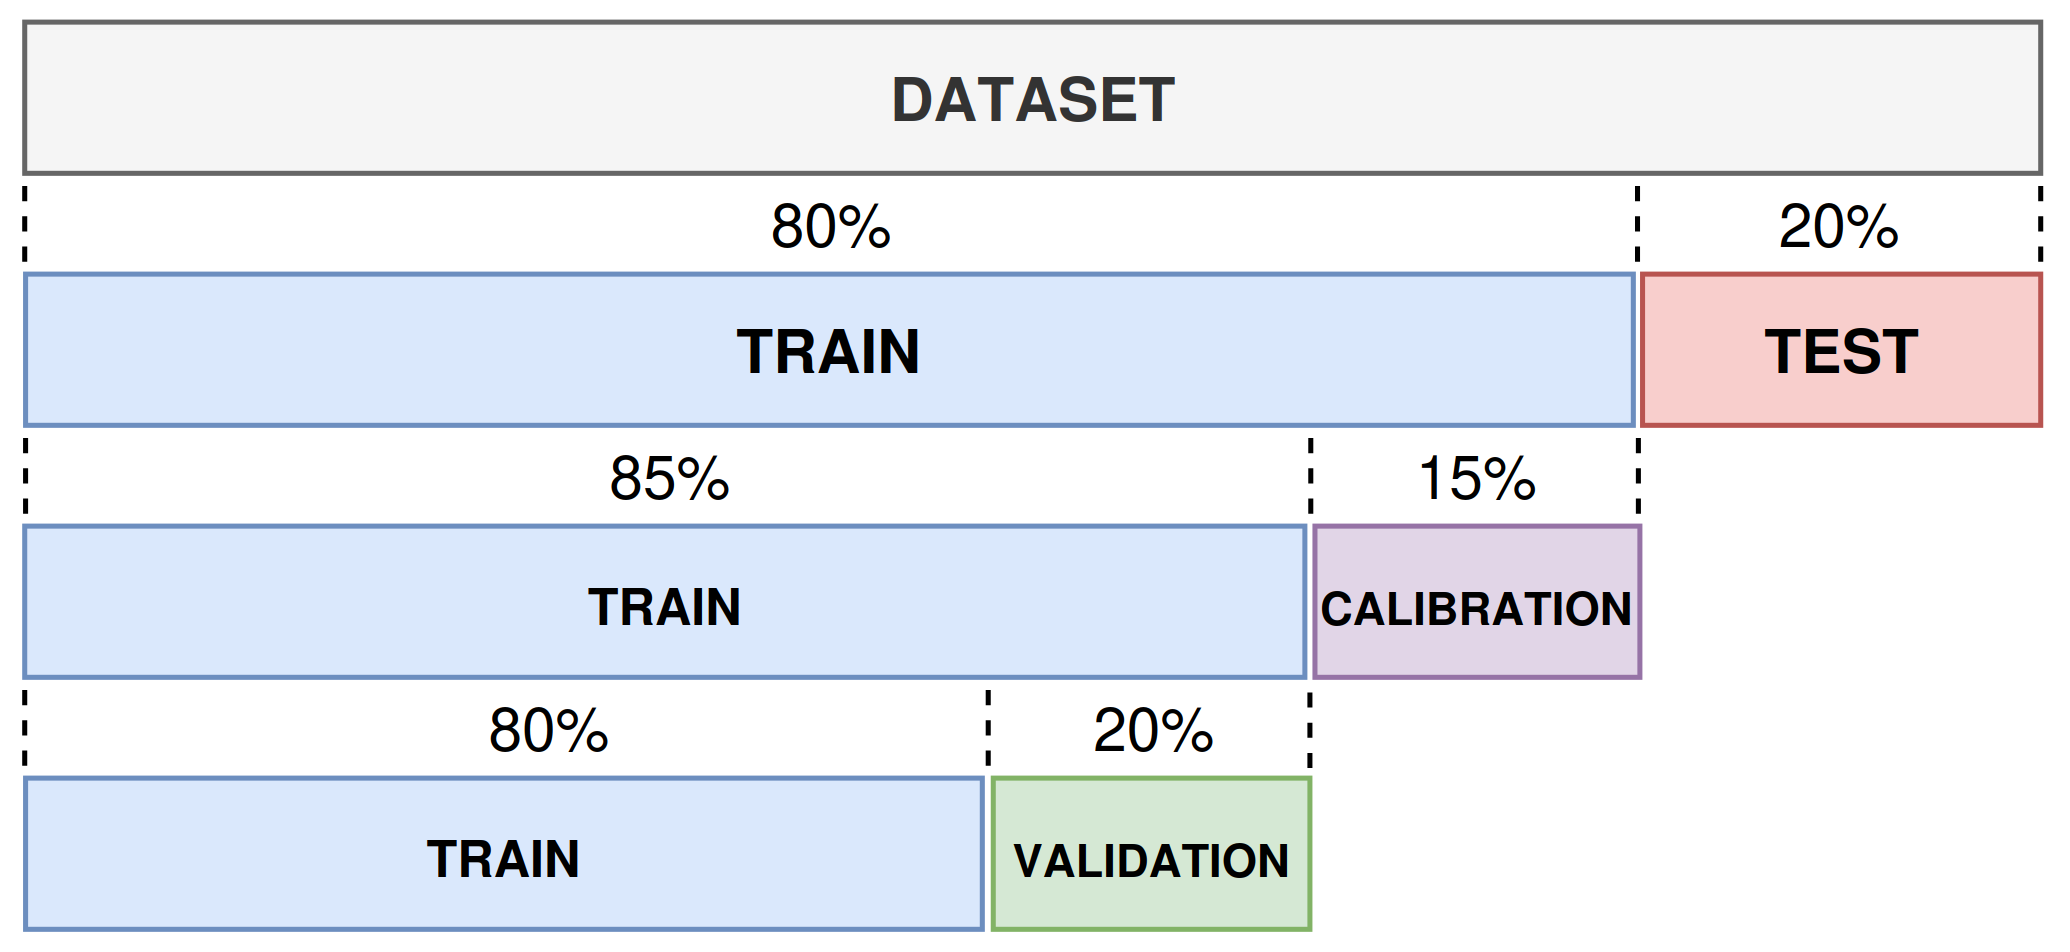
\includegraphics[width=\textwidth]{capitulos/cap_04/imagenes/data_split_conformal.png}
    \caption[
        Diagrama de división del \textit{dataset} en \textit{train}, \textit{validation}, \textit{calibration} 
        y \textit{test}.
    ]{
        Diagrama de división del \textit{dataset} en \textit{train}, \textit{validation}, \textit{calibration}
        y \textit{test}. Elaboración propia.
    } 
    \label{fig:data_split_conformal}
\end{figure}



% ------------------------------------------------------------------------------------------------------------

\section{Métricas}



% MAE
% MSE
% R² 

% Covertura empírica
% Tamaño intervalo medio

% ------------------------------------------------------------------------------------------------------------

\section{Experimentos realizados}

